\documentclass[10pt,conference]{IEEEtran}
\IEEEoverridecommandlockouts

\usepackage{cite}
\usepackage{amsmath,amssymb,amsthm}
\usepackage{graphicx}
\usepackage{tabularx}
\usepackage{booktabs}
\usepackage{xcolor}
\definecolor{visiblegray}{HTML}{CCCCCC}
\usepackage{listings}
\usepackage{url}
\usepackage{array}

\pagestyle{plain}
\pagenumbering{arabic}

\begin{document}

\title{LED-ML: Causal Lens of Layer-wise Energy Dissipation in LLM}

\author{\IEEEauthorblockN{Sudharsan Vijayaraghavan}
\IEEEauthorblockA{Independent Researcher}\\
Email: dlytiks@gmail.com
}
\maketitle

\begin{abstract}
This paper presents an observability mechanism for LLM internals that simultaneously captures forward activations and Vector-Jacobian Products (VJPs) of target output logits. It provides lightweight, hook based implementation designed to extract runtime tensors and target gradients safely across layers. A down-sampled subset of these captured tensors are rendered into text based visual maps and Graphics Interchange Format (GIF) animations. This framework provides an illustrative and intuitive interface for analyzing the internal states and semantic interpretations of deep models, enabling architecture debugging, training diagnostics, and dynamic routing.
\end{abstract}

\section{Introduction}

A visual telemetry of forward activations~\cite{paszke2019pytorch} and backward gradients of target logits~\cite{mu_mis2026remaining} is presented for the surgical observability of deep layer architectures. Post-attention~\cite{postln2026back} or post-feedforward layer normalizations~\cite{dead2026directions} alongside self-attention output projections are tracked to visualize forward activations and the top-$K$ neurons of each layer. In addition, a \textbf{Vector-Jacobian Product (VJP)}~\cite{goodfellow2016deep} ~\cite{bakong2026unbiased}  on the final target logit scalars is tracked for causal gradients to construct intuitive structural illustrations.

A hook-based approach on models for both the forward and backward pass makes it a plug-and-play solution to create text and GIF illustrations. A Python package \textbf{led-ml} is introduced, providing a simple means to overlay tracking hooks onto a given model during its execution. The forward and backward hooks run for every prompt, exposing a live visual map of the internal activations and targeted gradients.

There are two modes in this framework's implementation, namely \textbf{decision} and \textbf{trajectory} modes. The \textbf{decision} mode tracks activations and VJPs exclusively for the first predicted token. On the other hand, the \textbf{trajectory} mode dynamically tracks activations and target gradients across all sequentially predicted tokens.

Ultimately, a dynamic presentation of the internal firings of neurons across all internal layers acts as a causal lens for fine-grained debugging. This paradigm disrupts traditional debugging approaches that rely on dumping raw, dense model parameters and weights, which often appear to the engineer as an uninterpretable \textbf{numberpile}.

\section{Related Work}
This diagnostic Causal Lens LED is inspired by logit lens ~\cite{nostalgebraist2020logitlens} and J-lens~\cite{gurnee2026verbalizable}. The major difference is this low overhead: we use VJP instead of full Jacobians and it is plug and play via PyTorch hooks

\section{Mathematical Formulation of the Activation and VJP Tracking Hooks}
\subsection{Mathematical Formulation of the Dynamic Activation Tracking Hook}

The mathematical formulation of tracking system captures single-token hidden states, filters out tensors using adaptive thresholds, maps feature vector intensities, and binds structural neuron mappings directly to weight configurations.

\subsubsection*{1. Variables and Dimensions}
\begin{tabularx}{\linewidth}{@{} p{7em} X @{}}
    \toprule
    $\mathbf{X}_l$ & The forward pass activation tensor for layer $l$. \\
    \addlinespace
    $\mathbf{a}_l \in \mathbb{R}^d$ & The extracted last-token activation vector of hidden dimension $d$. \\
    \addlinespace
    $\Omega_l$ & The subset of neuron indices that pass adaptive noise thresholds, maps feature vector intensities, and binds structural neuron mappings directly to weight configurations. \\
    \addlinespace
    $\mathbf{v}_{\text{top}}, \mathbf{v}_{\text{bottom}} \in \mathbb{Z}^d$ & Sign-embedded vectors tracking top and bottom 30\% thresholds... \\
    \addlinespace
    $S_{\text{first}}, S_{\text{last}}$ & The flat 10\% visual sampling window sequences rendered... \\
    \addlinespace
    $\Psi_l$ & The index set containing the top $K=3$ absolute highest values, rendered with true sign... \\
    \bottomrule
\end{tabularx}
\medskip

\subsubsection*{2. Vector Extraction}
The forward hook intercepts the hidden state tensor and extracts the final sequence token vector from the first batch item:
\[
\mathbf{a}_l = \mathbf{X}_{l}[0, -1, :]
\]

\subsubsection*{3. Adaptive Noise Thresholding}
To filter out low-variance background noise, independent upper and lower floor boundaries are calculated dynamically:
\[
\tau_{\text{pos}} = \begin{cases} 0.3 \cdot \max(\mathbf{a}_l), & \text{if } \max(\mathbf{a}_l) > 0 \\ 0.0, & \text{otherwise} \end{cases}
\]
\[
\tau_{\text{neg}} = \begin{cases} 0.3 \cdot \min(\mathbf{a}_l), & \text{if } \min(\mathbf{a}_l) < 0 \\ 0.0, & \text{otherwise} \end{cases}
\]
Neuron indices clearing either boundary are admitted into the threshold activation set $\Omega_l$:
\[
\Omega_l = \left\{ j \in [0, d-1] \;\middle\vert{}\; \mathbf{a}_l(j) > \tau_{\text{pos}} \;\lor\; \mathbf{a}_l(j) < \tau_{\text{neg}} \right{}
\]
The global active density ratio per layer is formulated as:
\[
\text{Active \%} = \frac{|\Omega_l|}{d} \times 100
\]

\subsubsection*{4. Cumulative Quantile Segmentation \& Sign Mapping}
Let $\mathbf{a}_{\Omega_l}$ be the sub-vector containing only valid thresholded features. The 30th and 70th percentile cutoffs~\cite{paul2025quantile} ~\cite{nanoquant2026efficient} are derived from this filtered distribution:
\[
\begin{aligned}
q_{30} = \text{Quantile}(\mathbf{a}_{\Omega_l}, 0.3) \\
q_{70} = \text{Quantile}(\mathbf{a}_{\Omega_l}, 0.7)
\end{aligned}
\]
The sparse sign-tracking tensors $\mathbf{v}_{\text{top}}$ and $\mathbf{v}_{\text{bottom}}$ are initialized to $\mathbf{0} \in \mathbb{R}^d$ and populated based on structural percentiles:
\paragraph{Top 30\% Bucket Map:}
\[
\mathbf{v}_{\text{top}}(j) = \begin{cases}  1, & \text{if } j \in \Omega_l \;\land\; \mathbf{a}_l(j) \ge q_{70} \;\land\; \mathbf{a}_l(j) \ge 0 \\  -1, & \text{if } j \in \Omega_l \;\land\; \mathbf{a}_l(j) \ge q_{70} \;\land\; \mathbf{a}_l(j) < 0 \\  0, & \text{otherwise}  \end{cases}
\]
\paragraph{Bottom 30\% Bucket Map:}
\[
\mathbf{v}_{\text{bottom}}(j) = \begin{cases}  1, & \text{if } j \in \Omega_l \;\land\; \mathbf{a}_l(j) \le q_{30} \;\land\; \mathbf{a}_l(j) \ge 0 \\  -1, & \text{if } j \in \Omega_l \;\land\; \mathbf{a}_l(j) \le q_{30} \;\land\; \mathbf{a}_l(j) < 0 \\  0, & \text{otherwise}  \end{cases}
\]

\subsubsection*{5. Visual 10\% Window Character String Rendering}
The window size for a flat 10\% sample is defined by $m = \max(1, \lfloor 0.10 \cdot d \rfloor)$. Boundary vectors are sliced and mapped to string sequences using the character transformation function $f(s)$:
\[
\begin{aligned}
S_{\text{first}} = \Big[ f\big(\mathbf{v}_{\text{top}}(j)\big) \Big]_{j=0}^{m-1} \\
S_{\text{last}} = \Big[ f\big(\mathbf{v}_{\text{bottom}}(j)\big) \Big]_{j=d-m}^{d-1}
\end{aligned}
\]
\[
 f(s) = \begin{cases} 
 \textcolor{green}{\blacktriangle}, & \text{if } s = 1 \quad \text{(Active Positive)} \\ 
 \textcolor{red}{\blacktriangledown}, & \text{if } s = -1 \quad \text{(Active Negative)} \\ 
 \textcolor{visiblegray}{\blacksquare}, & \text{if } s = 0 \quad \text{(Inactive)} 
 \end{cases}
\]
The density counts within these discrete tracking windows are calculated using the indicator function $\mathbb{I}$:
\begin{aligned}
\text{Count}_{\text{first}} &= \frac{1}{m} \sum_{j=0}^{m-1} \mathbb{I}\left(\mathbf{v}_{\text{top}}(j) \neq 0\right) \\[1ex]
\text{Count}_{\text{last}}  &= \frac{1}{m} \sum_{j=d-m}^{d-1} \mathbb{I}\left(\mathbf{v}_{\text{bottom}}(j) \neq 0\right)
\end{aligned}

\subsubsection*{6. Structural Top-$K$ Neuronal Profiling}
The model isolates the structural identities of the top $K=3$ absolute highest-magnitude neurons, uses true value to display the signs of magnitude:
\[
\Psi_l = \text{arg\,top-3}\left( \left| \mathbf{a}_l(j) \right| \right)
\]
For each dominant neuron index $i \in \Psi_l$, structural weight profiles are extracted safely without gradient tracking based on the sub-module target configuration:
\paragraph{Case A: Normalization Parameter Weights (\texttt{norm\_attr})}
\[
\begin{aligned}
\text{weight\_norm}_i &= \|\mathbf{w}(i)\|_2 = |\mathbf{w}(i)| \\[1ex]
\text{where } \mathbf{w} &\in \mathbb{R}^d, \quad i < \text{dim}(\mathbf{w})
\end{aligned}
\]

\paragraph{Case B: Attention Matrix Layer Weights (\texttt{attn\_attr})}
\[
\text{top\_input\_weights}_i = \text{top-3}\left( \left| \mathbf{w}_i \right| \right) \quad \text{where } \mathbf{w}_i = \mathbf{W}[:, i] \in \mathbb{R}^{d_{\text{in}}}
\]

\subsubsection*{7. Relational Database Serialization Map}
At execution step $t$ for layer $l$, the metrics are committed to the global tracking matrix storage engine $\mathcal{D}(t, l)$:
\[
\mathcal{D}(t, l) = \left\{ \text{"Forward\_Activations"}: \begin{bmatrix} S_{\text{first}} \\ S_{\text{last}} \\ \text{Count}_{\text{first}} \\ \text{Count}_{\text{last}} \\ \text{Active \%} \\ \left\{ \big(i, |\mathbf{a}_l(i)|, \text{source}, \mathcal{W}_i\big) \;\middle\vert{}\; i \in \Psi_l \right\} \end{bmatrix} \right\}
\]
\[
\text{where } \mathcal{W}_i = \begin{cases} \text{weight\_norm}_i, & \text{if module matches } \textit{norm\_attr} \\ \text{top\_input\_weights}_i, & \text{if module matches } \textit{attn\_attr} \end{cases}
\]

\subsection{Mathematical Formulation of the VJP Backward Tensor Hook}
\subsubsection*{1. Backward VJP Trigger Mechanism}
The backward tracking workflow isolates a specific target logit coordinate to propagate gradients. Let $\mathbf{y} \in \mathbb{R}^V$ represent the model output logit vector for the final sequence token across vocabulary size $V$. Given a specific target token index $k \in [0, V-1]$, the scalar objective function $J$ is defined as:
\[
J = \mathbf{y}(k)
\]
The reverse-mode automatic differentiation execution is triggered by computing the scalar derivative:
\[
\frac{\partial J}{\partial J} = 1
\]
This backpropagation computes the Vector-Jacobian Product (VJP) across preceding layers. For a tracking target hidden state vector $\mathbf{h}_l$, the hook intercepts the upstream structural gradient vector $\mathbf{g}_l \in \mathbb{R}^d$:
\[
\mathbf{g}_l = \frac{\partial J}{\partial \mathbf{h}_l} = \left[ \frac{\partial \mathbf{y}(k)}{\partial \mathbf{h}_l(0)}, \frac{\partial \mathbf{y}(k)}{\partial \mathbf{h}_l(1)}, \dots, \frac{\partial \mathbf{y}(k)}{\partial \mathbf{h}_l(d-1)} \right]
\]

\subsubsection*{2. Gradient Extraction}
The backward tensor hook ~\cite{paszke2017automatic} isolates the structural spatial gradient vector corresponding to the final token sequence length entry from the primary batch item:
\[
\mathbf{g}_l = \boldsymbol{\nabla}_{\mathbf{h}_l} J = \mathbf{G}_{l}[0, -1, :]
\]

\subsubsection*{3. Instantaneous Gradient Noise Thresholding}
To measure structural gradient sensitivity while ignoring low-magnitude variance, an magnitude vector $|\mathbf{g}_l|$ is calculated. A dynamic noise cutoff floor $\gamma_l$ is derived using the upper 30\% bound of peak gradient intensity:
\[
\gamma_l = 0.3 \cdot \max_{j} \left| \left \mathbf{g}_l(j) \right|
\]
A binary indicator state vector $\mathbf{b}_l \in \{0, 1\}^d$ maps elements clearing this dynamic threshold:
\[
\mathbf{b}_l(j) = \begin{cases} 1, & \text{if } \left| \mathbf{g}_l(j) \right| > \gamma_l \\ 0, & \text{otherwise} \end{cases}
\]
The overall gradient activation percentage across the hidden dimension $d$ is given by:
\[
\text{Grad Active \%} = \frac{\sum_{j=0}^{d-1} \mathbf{b}_l(j)}{d} \times 100
\]

\subsubsection*{4. Flat 10\% Gradient Window \& Block LED Rendering}
A fixed spatial window boundary constraint is computed as $m = \max(1, \lfloor 0.10 \cdot d \rfloor)$. Slices tracking the beginning and end of the binary indicators are transformed into a character visualization sequence using the state rendering function $g(b)$:
\[
S_{\text{grad\_first}} = \Big[ g\big(\mathbf{b}_l(j)\big) \Big]_{j=0}^{m-1}, \quad S_{\text{grad\_last}} = \Big[ g\big(\mathbf{b}_l(j)\big) \Big]_{j=d-m}^{d-1}
\]
\[
g(b) = \begin{cases} \textcolor{green}{\blacksquare}, & \text{if } b = 1 \quad \text{(Active Gradient)} \\ \textcolor{visiblegray}{\blacksquare}, & \text{if } b = 0 \quad \text{(Inactive Gradient)} \end{cases}
\]
The discrete density tracking metrics are captured via fractional ratio strings:
\[
\begin{aligned}
\text{Grad Count}_{\text{first}} &= \frac{\sum_{j=0}^{m-1} \mathbf{b}_l(j)}{m} \\
\text{Grad Count}_{\text{last}} &= \frac{\sum_{j=d-m}^{d-1} \mathbf{b}_l(j)}{m}
\end{aligned}
\]

\subsection{Combined Metrics Serialization Map}
The tracking engine appends these backpropagation parameters directly into the step $t$ and layer $l$ structural storage block alongside forward state entries:
\[
\mathcal{D}(t, l) = \left\{ \begin{aligned}
&\text{"Forward\_Activations"}: \mathbf{V}_{\text{fwd}}, \\
&\text{"Backward\_Grads"}: \mathbf{V}_{\text{bwd}}
\end{aligned} \right\}
\]

\[
\mathbf{V}_{\text{bwd}} = [ \mathbf{S}^T, \mathbf{C}^T, \text{Grad Active \%} ]^T
\]

\[
\text{where } \mathbf{S} = \begin{bmatrix} S_{\text{grad\_first}} \\ S_{\text{grad\_last}} \end{bmatrix}
\]

\[
\text{and } \mathbf{C} = \begin{bmatrix} \text{Grad Count}_{\text{first}} \\ \text{Grad Count}_{\text{last}} \end{bmatrix}
\]

\section{Telemetry Rendering}
\subsection*{1. Text Telemetry Renderer}
The serialization architecture outputs structured ASCII matrices directly to the console stream using a tracking function \texttt{text\_led}. Let $\mathcal{D}$ be the execution metrics database block, $L$ be the total layers, and $T_{\text{steps}}$ be the total token generation sequence length steps. 

For each individual prediction step $t \in [0, T_{\text{steps}}-1]$, the telemetry matrix loops sequentially over all operational layout blocks to print structural string columns.

\paragraph*{a) Structured String Alignment Constraints}
The character visualization strings are aligned with padding to preserve hidden feature spatial coordinates across disparate terminals. Let $c$ represent the minimum character column constraint calculated dynamically from the 10\% hidden vector dimension window. Slices are formatted via padding transformations:
\[
\begin{aligned}
\text{Output}_{\text{Forward}} &= \text{Pad}_{\text{Left}}\Big(S_{\text{first}}, 45\Big) \\
\text{Output}_{\text{Jacobian}} &= \text{Pad}_{\text{Left}}\Big(S_{\text{grad\_first}}, 45\Big)
\end{aligned}
\]

\paragraph*{b) Multi-Layer Component Execution Loop}
\begin{sloppypar}
The printing framework iterates uniformly over layer indices $l \in [0, L-1]$ to decouple component tables. The operational workflow executes the following display sequences:
\end{sloppypar}

\begin{enumerate}
    \item \textbf{Token Context Definition}: Prints target token step index $t$ alongside the decoded string prediction token scalar.
    \item \textbf{Forward Map Slicing}: Outputs the 45-column left-padded forward activation window symbol strings ($S_{\text{first}}$, $S_{\text{last}}$) matching layer coordinate $l$, followed by the fractional density ratio indicator string.
    \item \textbf{Jacobian Map Slicing}: Outputs the 45-column left-padded causal sensitivity VJP gradient symbol strings ($S_{\text{grad\_first}}$, $S_{\text{grad\_last}}$) along with the active gradient integer tracking ratio string.
    \item \textbf{Density Matrix Compression}: Projects a summary sub-table displaying side-by-side scalar percentages mapping layer active densities:
    \[
    \text{Row}_l = \Big[ l, \; \text{Active \%}_l, \; \text{Grad Active \%}_l \Big]
    \]
    \item \textbf{Runtime Performance Overhead Profiling}: Extracts individual runtime layer latency anomalies ($\Delta \tau_l$) introduced by forward and backward tracking hook operations:
    \[
    \text{Overhead}_t = \Delta \tau_l \quad \text{(measured in milliseconds)}
    \]
    \item \textbf{Top-$K$ Parameters Serialization}: Prints a serialized JSON string containing structured coordinate indices, magnitudes, and layer attribution weights for the top 3 absolute highest-energy neurons:
    \[
    \text{JSON}_l = \left\{ \big(i, |\mathbf{a}_l(i)|, \text{source}, \mathcal{W}_i\big) \;\middle\vert{}\; i \in \Psi_l \right\}
    \]
\end{enumerate}

\subsection*{2. Multi-Frame Graphical Telemetry (GIF Rendering Engine)}
To capture temporal execution dependencies across sequential generation tokens, the framework implements a dual-stream visual serialization pipeline via the function \texttt{gif\_led}. This routine accepts the step-indexed dictionary database $\mathcal{D}$ and constructs two distinct Graphics Interchange Format (GIF)~\cite{compuserve1987gif87a} visual maps concurrently.

\paragraph{Structural Data Extraction and Coordinate Mapping}
Let $T_{\text{steps}}$ be the total token generation steps, and $L$ be the total deep layers. For each prediction interval $t \in [0, T_{\text{steps}}-1]$, structural character symbols are collected across all layer coordinates $l \in [0, L-1]$. The maximum sequence layer width bounds are determined dynamically by:
\[
W_{\text{max}} = \max_{t, l} \left( \text{length}\Big(S_{\text{first}}(t, l) \mathbin{\parallel} S_{\text{last}}(t, l)\Big) \right)
\]
Where $\mathbin{\parallel}$ represents the string concatenation operator. The engine routes this extracted structural text stream down two isolated parsing pipelines to build independent frame matrices:

\begin{enumerate}
    \item \textbf{Text Overlay Grid Mapping} ($\mathbf{M}_{\text{std}}$): Characters are left-padded or truncated to a fixed horizontal viewing span of exactly 100 column slices to preserve geometric terminal boundaries:
    \[
    \mathbf{M}_{\text{std}}(l) = \text{Slice}_{100}\Big(S_{\text{first}}(t, l) \mathbin{\parallel} S_{\text{last}}(t, l) \mathbin{\parallel} \text{" "}^{100}\Big)
    \]
    Where the scalar mapping function evaluates state codes as:
    \[
    \phi(c) = \begin{cases} 
    0, & \text{if } c = \textcolor{visiblegray}{\blacksquare} \quad \text{(Inactive Background)} \\ 
    1, & \text{if } c = \textcolor{green}{\blacksquare} \quad \text{(Active Core Element)} \\ 
    2, & \text{if } c = \textcolor{green}{\blacktriangle} \quad \text{(Active Positive Forward pass)} \\ 
    3, & \text{if } c = \textcolor{red}{\blacktriangledown} \quad \text{(Active Negative pass)} 
    \end{cases}
    \]
    \item \textbf{Discrete Numeric Pixel Mapping} ($\mathbf{M}_{\text{extended}}$): String sequences are padded up to $W_{\text{max}}$ and transformed into a numeric coordinate space using a discrete mapping operator $\phi(c)$:
    \[
    \mathbf{M}_{\text{extended}}(l, x) = \phi\Big( \big[S_{\text{first}}(t, l) \mathbin{\parallel} S_{\text{last}}(t, l) \mathbin{\parallel} \text{" "}^{W_{\text{max}}}\big]_x \Big)
    \]
    Where the scalar mapping function evaluates state codes as:
    \[
    \phi(c) = \begin{cases} 
    0, & \text{if } c = \textcolor{visiblegray}{\blacksquare} \quad \text{(Inactive Background)} \\ 
    1, & \text{if } c = \textcolor{green}{\blacksquare} \quad \text{(Active Core Element)} \\ 
    2, & \text{if } c = \textcolor{green}{\blacktriangle} \quad \text{(Active Positive Forward pass)} \\ 
    3, & \text{if } c = \textcolor{red}{\blacktriangledown} \quad \text{(Active Negative pass)} 
    \end{cases}
    \]
\end{enumerate}

\paragraph{Dual-Stream Plot Rendering Configurations}
The standard visualization canvas renders a side-by-side subplot tracking the \textit{Forward Activations Profile} and the \textit{Jacobian Causal Sensitivity (VJP)}

\subparagraph{1. Standard Character Overlay Visualization:}
The standard visualization at a target resolution of 110 dots per inch (DPI).  The numeric frame matrix $\mathbf{M}_{\text{std}}$ is mapped directly to individual pixels

\subparagraph{2. High-Resolution Numeric Pixel Matrix View:}
The extended pixel matrix canvas utilizes a high-resolution layout configured at 130 DPI to show fine-grained architectural patterns. The numeric frame matrix $\mathbf{M}_{\text{extended}}$ is mapped directly to individual pixels

\paragraph{C. Simultaneous Multi-Frame Image Compiling}
Let $F_{\text{fps}}$ define the desired visualization frame rate. Individual frame canvas buffers are captured sequentially in memory and stacked into a final animated image sequence. The inter-frame display delay parameter $\Delta T_{\text{frame}}$ is calculated in milliseconds as:
\[
\Delta T_{\text{frame}} = \left\lfloor \frac{1000}{F_{\text{fps}}} \right\rfloor
\]
The final image compiling loop packages all independent temporal frames sequentially to output two separate multi-frame graphical files simultaneously:
\[
\text{File}_{\text{standard}} = \mathbf{\Phi}_{\text{save}}\left( \mathbf{M}_{\text{std}}(0), \dots, \mathbf{M}_{\text{std}}(T_{\text{steps}}-1), \; \Delta T_{\text{frame}} \right)
\]
\[
\text{File}_{\text{extended}} = \mathbf{\Phi}_{\text{save}}\left( \mathbf{M}_{\text{extended}}(0), \dots, \mathbf{M}_{\text{extended}}(T_{\text{steps}}-1), \; \Delta T_{\text{frame}} \right)
\]
Where $\mathbf{\Phi}_{\text{save}}$ represents the multi-frame compilation function operating with infinite animation looping enabled.
The sample visual maps are provided in APPENDIX ~\ref{app:visual_maps}
\section{Operational Modes Workflow}

\subsubsection{Decision Mode}
This mode captures activations and VJPs of all layers for the first predicted token only. This sets the tone of capture since it decides the prediction pattern while responding for a prompt.

\subsubsection{Trajectory Mode}
This mode captures activations and VJPs of all layers for the all predicted tokens. The capture shows the sequence of actions for the entire response

\section{Hook latency}
The following is captured for the hook for every layer. It is imperative to mention the hook will add a latency and Trajectory mode runs hooks for every new token generated upto 128 new tokens
 \[
    \text{Overhead}_t = \Delta \tau_l \quad \text{(measured in milliseconds)}
 \]

\section{Software Implementation and API Architecture}
\label{sec:software_implementation}

The proposed observability framework is implemented as an open-source, production-ready Python package titled \textbf{\texttt{led-ml}}\footnote{Available on the Python Package Index (PyPI) and GitHub at \url{https://github.com/dlytik/led-ml}}. The library functions by dynamically registering PyTorch forward layer hooks across target hidden states alongside backward tensor hooks on the target output logits to capture precise Vector-Jacobian Products (VJPs) with minimal runtime overhead. 

The core operational workflow of the \texttt{led-ml} API exposes the following structural methods for user orchestration:

\begin{description}
    \item[\texttt{led\_ml.led\_core}] \hfill \\
    Initializes the primary telemetry core instance, anchoring the tracking state, target model configurations
    
    \item[\texttt{get\_supported\_models()}] \hfill \\
    Queries and returns a validated registry of deep learning transformer architectures currently supported for inline telemetry extraction.
    
    \item[\texttt{run\_model(model, prompt, ...)}] \hfill \\
    Executes a contextual inference step on the wrapped model object, automatically handling the orchestration, triggering, and safe teardown of the forward/backward tracking hooks during execution.
    
    \item[\texttt{get\_led()}] \hfill \\
    Extracts the compiled internal telemetry metrics directly from the tracking buffer, returning the structural tensor data and VJP outputs as a native Python dictionary.
    
    \item[\texttt{text\_led()}] \hfill \\
    Serializes and formats the raw internal tensor matrices into a down-sampled, highly scannable, text-based visual map directly inside the terminal layout.
    
    \item[\texttt{gif\_led()}] \hfill \\
    Compiles the spatio-temporal layers and sequential token trajectories from the telemetry buffer, rendering them into a smooth Graphics Interchange Format (GIF) animation for localized dashboard visual inspection.

    \item[\texttt{lat\_led()}] \hfill \\
    Captures and calculates the mean ($\mu$) and standard deviation ($\sigma$) of latencies for every layer across all tokens for a given query.

    \item[\texttt{ram\_led()}] \hfill \\
    Captures size of the entire led object in $MB$ for a given query.

\end{description}

\section{Limitations}
Tensor parallelism ~\cite{santopaolo2026tensor} is not supported as part of forward hook yet. Hooks will add latency noticeable in Trajectory mode if the there lots of layers. Telemetry object consumes storage proportional to number of layers and mode chosen for inspection

A primary computational limitation of the current framework lies in its sequence generation efficiency during diagnostic parsing. The existing implementation does not utilize Key-Value (KV) caching mechanisms, which introduces a strict memory-access and computational bottleneck that forces the autoregressive decoding phase into a quadratic time complexity of $\mathcal{O}(T^2)$, where $T$ denotes the sequence length. Further for every new token generation, the forward pass starts from zeroth token index, which makes it $\mathcal{O}(T^3)$

To maintain mathematical transparency for Vector-Jacobian Product (VJP) tracking, computing independent backward passes sequentially across tokens was prioritised over production-level inference optimizations. In the next iteration, this architecture will be optimized to alleviate the latency wall. Future work will target linear-time decoding while preserving per-token gradient tracing for full trajectory mapping.


\section{Future Work}
\label{sec:future_work}
The following phases will be explored.
\begin{enumerate}
    \item \textbf{Optimization for speed:} We intend to optimize the repeated zeroth token index starting forward pass for every new token generation. Key-Value cache using \texttt{past\_key\_values} will be attempted to solve quadratic time complexity.

    \item \textbf{Topological Classification of Empirical Model Inertia:} We intend to leverage the \textit{trajectory mode} of \texttt{led-ml} to formally characterize model inertia across diverse semantic workloads. This will isolate depth zones where the forward hidden state updates diminish ($\Delta H_l \to 0$) alongside vanishing logit-specific VJPs, identifying exact architectural layer blocks where the model achieves consensus or hits computational representation plateaus.
    
    \item \textbf{Profiling Token-Level Resistance Mechanics:} Future work will systematically profile model \textit{resistance} by isolating layers that yield dense, high-magnitude negative Vector-Jacobian Products ($J^T v \ll 0$). Characterizing these inhibitory gradients will map the internal boundaries where specific layers actively suppress counterfactual tokens, revealing the structural pathways models use to veto alternative causal paths during generation.
    
    \item \textbf{Deriving a Unified Layer Efficiency Index:} Using the mapped spatial distributions of both forward inertia and backward resistance across the network stack, we aim to construct a unified metric for model efficiency. This optimization framework will evaluate whether structural layers are computationally over-parametrized for a given query type, guiding downstream layer-pruning and adaptive execution pipelines based on raw telemetry rather than static weight analysis.
    
    \item \textbf{Causal Layer Fingerprinting of Deep Architectures:} By capturing the unique spatial and temporal patterns of activations and VJPs across model families, we propose the creation of diagnostic ``model fingerprints.'' These low-dimensional, text- and GIF-rendered profiles will serve as distinct operational signatures, allowing engineers to uniquely identify, audit, and compare model variants and fine-tuning states without inspecting raw weight distributions or dense parameter repositories.

\end{enumerate}

\section{Conclusion}
The paper showcases an intuitive way to visualise internals of LLM layers (activations and VJP on target logits) moving away from traditional numbers which is a nightmare to articulate and understand. 

The introduction of VJP enables an extremely light weight one backward pass after prediction to identify relevant gradients. The activations are collected in forward pass one the go with very low overhead which makes it perfect for identifying inertia and resistance of model predictions.

\newpage
\bibliographystyle{IEEEtran}
\bibliography{references}

\newpage
\appendices

\section{Granular Layer-wise Hook Latency Telemetry}
\label{appendix:latency_telemetry}

To evaluate the exact computational overhead introduced by our tracking framework, we record the execution duration of our forward hooks across deep layer boundaries. Telemetry is collected for every individual layer $N$ across all generated tokens $M$ during inference. 

Table~\ref{tab:layer_latencies_detailed} presents the detailed profile. For each layer row, the reported metrics reflect the mean latency ($\mu$) and standard deviation ($\sigma$) calculated across the entire generation sequence length ($M = 10$ for Qwen2, $M = 111$ for Mistral, and $M = 74$ for OpenChat). This layout isolates structural variances and demonstrates that tracking overhead remains low and uniform across both shallow and deep transformer layers.
Timings reported are indicative hook overhead on 15-core heterogeneous ARM64 processor at 4.6~GHz with 24~GB memor. LED is a diagnostic tool; absolute latency varies with prompt, batch size, and hardware. We do not report SOTA numbers
\begin{table}[htbp]
\centering
\caption{Layer-by-Layer Hook Latency Profiling (Values in Milliseconds)\protect\footnotemark}
\label{tab:layer_latencies_detailed}
\begin{tabular}{cccc}
\toprule
\textbf{Layer} & \textbf{Qwen2-7B} & \textbf{Mistral-7B} & \textbf{OpenChat-3.5} \\
\textbf{Index} & ($M=10$ Tokens) & ($M=111$ Tokens) & ($M=74$ Tokens) \\
\midrule
Layer 1  & $29.33 \pm 24.03$ & $71.96 \pm 49.17$ & $61.96 \pm 49.77$ \\
Layer 2  & $15.53 \pm 2.86$ & $29.14 \pm 22.02$ & $42.91 \pm 48.95$ \\
Layer 3  & $14.10 \pm 4.65$ & $24.07 \pm 15.97$ & $25.75 \pm 23.55$ \\
Layer 4  & $13.86 \pm 2.96$ & $24.22 \pm 20.83$ & $22.33 \pm 17.19$ \\
Layer 5  & $17.86 \pm 7.05$ & $31.34 \pm 38.35$ & $23.47 \pm 11.98$ \\
Layer 6  & $16.92 \pm 7.22$ & $22.16 \pm 11.68$ & $22.42 \pm 10.67$ \\
Layer 7  & $17.94 \pm 6.89$ & $58.85 \pm 56.25$ & $34.74 \pm 32.41$ \\
Layer 8  & $16.51 \pm 3.12$ & $26.20 \pm 15.41$ & $32.07 \pm 42.03$ \\
Layer 9  & $22.91 \pm 26.86$ & $26.07 \pm 18.16$ & $37.71 \pm 47.00$ \\
Layer 10 & $18.41 \pm 5.34$ & $115.57 \pm 71.76$ & $53.52 \pm 62.19$ \\
Layer 11 & $30.40 \pm 35.36$ & $31.12 \pm 29.56$ & $38.03 \pm 27.84$ \\
Layer 12 & $18.38 \pm 7.19$ & $92.29 \pm 64.36$ & $30.80 \pm 21.13$ \\
Layer 13 & $20.24 \pm 8.37$ & $29.87 \pm 24.73$ & $39.70 \pm 41.38$ \\
Layer 14 & $26.73 \pm 23.00$ & $30.62 \pm 30.10$ & $32.58 \pm 30.53$ \\
Layer 15 & $21.78 \pm 24.21$ & $37.38 \pm 40.62$ & $32.52 \pm 33.41$ \\
Layer 16 & $27.86 \pm 30.48$ & $32.35 \pm 34.25$ & $31.44 \pm 31.23$ \\
Layer 17 & $22.44 \pm 22.28$ & $68.18 \pm 54.59$ & $41.25 \pm 30.51$ \\
Layer 18 & $19.14 \pm 12.73$ & $30.91 \pm 31.43$ & $31.43 \pm 32.28$ \\
Layer 19 & $16.38 \pm 4.86$ & $29.97 \pm 28.29$ & $34.09 \pm 35.32$ \\
Layer 20 & $53.85 \pm 61.27$ & $29.39 \pm 25.35$ & $30.45 \pm 30.44$ \\
Layer 21 & $16.36 \pm 4.47$ & $35.20 \pm 34.20$ & $30.45 \pm 30.44$ \\
Layer 22 & $17.23 \pm 6.98$ & $61.18 \pm 35.00$ & $31.19 \pm 32.28$ \\
Layer 23 & $15.47 \pm 3.37$ & $83.85 \pm 96.10$ & $28.23 \pm 17.54$ \\
Layer 24 & $24.28 \pm 23.59$ & $72.05 \pm 69.57$ & $36.64 \pm 43.51$ \\
Layer 25 & $15.60 \pm 4.23$ & $36.62 \pm 27.02$ & $40.39 \pm 47.95$ \\
Layer 26 & $14.92 \pm 5.40$ & $38.83 \pm 40.18$ & $34.25 \pm 26.64$ \\
Layer 27 & $45.76 \pm 54.02$ & $56.90 \pm 45.86$ & $29.70 \pm 45.11$ \\
Layer 28 & $22.59 \pm 14.29$ & $46.24 \pm 50.10$ & $30.69 \pm 22.57$ \\
Layer 29 & \multicolumn{1}{c}{---} & $50.66 \pm 56.69$ & $31.66 \pm 35.54$ \\
Layer 30 & \multicolumn{1}{c}{---} & $36.15 \pm 35.15$ & $29.86 \pm 29.00$ \\
Layer 31 & \multicolumn{1}{c}{---} & $27.03 \pm 19.53$ & $33.39 \pm 32.84$ \\
Layer 32 & \multicolumn{1}{c}{---} & $48.78 \pm 45.73$ & $25.30 \pm 18.22$ \\
Layer 32 & \multicolumn{1}{c}{---} & $0.18 \pm 0.04$ & $30.87 \pm 26.77$ \\
\bottomrule
\end{tabular}
\end{table}
\footnotetext{All profiling metrics recorded using the evaluation input prompt: \texttt{"What is color of chlorophyll?"}}

\section{Layer-wise Metrics Schema Specification}
\label{appendix:schema_telemetry}

To formalize the tracking capabilities of the framework, we map out the complete diagnostic schema structure in Table~\ref{tab:telemetry_schema}. This explicitly lists the data types and metric contexts collected concurrently via our forward activation layers and VJP gradient vector hooks.
\begin{table*}[htbp]
\centering
\caption{Causal Lens LED Diagnostic Telemetry Schema Structure}
\label{tab:telemetry_schema}
\begin{tabular}{lll}
\toprule
\textbf{Field / Object Path Reference} & \textbf{Data Type} & \textbf{Logical Metric / Architectural Description} \\
\midrule
\texttt{prompt} & String & Raw text input evaluation sequence context. \\
\texttt{model} & String & Target architecture configuration name (e.g., Mistral-7B). \\
\texttt{torch\_dtype} & String & torch data type (e.g., torch.float16). \\
\texttt{mode} & String & Tracking environment functional run flags. \\
\texttt{num\_layers} & Integer & Total structural transformer layer count ($N$). \\
\texttt{ten\_pct\_cnt} & Integer & 10\% baseline token sequence index margin constraint. \\
\midrule
\multicolumn{3}{l}{\textbf{Per Generated Token Block} (\texttt{"0"} to \texttt{"M-1"})}\\
\midrule
\texttt{\ \ [Token ID]/target} & String & Actual decoded vocabulary target text prediction word. \\
\midrule
\multicolumn{3}{l}{\textbf{\ \ $\rightarrow$ Per Layer Structural Tracking Matrix Sub-Block} (\texttt{"0"} to \texttt{"N-1"})}\\
\midrule
\texttt{\ \ \ \ [Layer ID]/hook\_overhead\_ms} & Float & Live operational layer forward hook execution latency profile. \\
\texttt{\ \ \ \ [Layer ID]/Forward\_Activations} & Dictionary & Compiled activation mapping metrics and top-$K$ indices. \\
\texttt{\ \ \ \ [Layer ID]/Backward\_Grads} & Dictionary & Compiled Vector-Jacobian Product (VJP) gradient vectors. \\
\midrule
\multicolumn{3}{l}{\textbf{\ \ \ \ \ \ $\rightarrow$ Nested Feature Profile Arrays} (Inside Activations / Gradients Group)}\\
\midrule
\texttt{\ \ \ \ \ \ .../map\_first\_per} & String & Structural token representation tracking array ($\mu$ head window). \\
\texttt{\ \ \ \ \ \ .../map\_last\_per} & String & Segmented structural tracking matrix array tail signature. \\
\texttt{\ \ \ \ \ \ .../count\_first\_str} & String & Quantitative metrics tracker index header string tracking. \\
\texttt{\ \ \ \ \ \ .../count\_last\_str} & String & Quantitative metrics tracker index tail string tracking. \\
\texttt{\ \ \ \ \ \ .../pct} & Float & Calculated structural density contribution ratio metrics. \\
\texttt{\ \ \ \ \ \ .../top\_neurons} & JSON-String & Serialized data array containing top-$K$ dominant active tracking indices. \\
\bottomrule
\end{tabular}
\end{table*}

\clearpage

\section{In-Memory RAM Footprint Profiles}
\label{appendix:ram_telemetry}

We evaluate the deep live memory object overhead generated right out of our extraction functions. Table~\ref{tab:ram_usage} outlines the peak RAM footprints measured across our evaluation target workloads. This validates that tracking detailed token diagnostics does not risk system memory starvation during long autoregressive context execution runs.

\begin{table}[htbp]
\centering
\caption{Peak RAM Usage of Telemetry Tracking Dictionary in Trajectory mode}
\label{tab:ram_usage}
\begin{tabular}{cccc}
\toprule
\textbf{Model} & \textbf{N Layers} & \textbf{M Tokens} & \textbf{Peak RAM} \\
\midrule
Qwen2-7B & 28 & 10 & 1.29\,MB \\
Mistral-7B & 32 & 111 & 17.57\,MB \\
OpenChat-3.5 & 32 & 74 & 11.82\,MB \\
\bottomrule
\end{tabular}
\end{table}

\section{Visual Feature Activation Map and Causal VJP}
\label{app:visual_maps}
This section provides a sample frame for visual analysis of the internal mechanics of OpenChat-3.5
The complete GIF animation for all tokens is provided in our repository; for the URL and implementation details, please refer to Section~\ref{sec:software_implementation}.

\begin{figure*}[htbp]
    \centering
    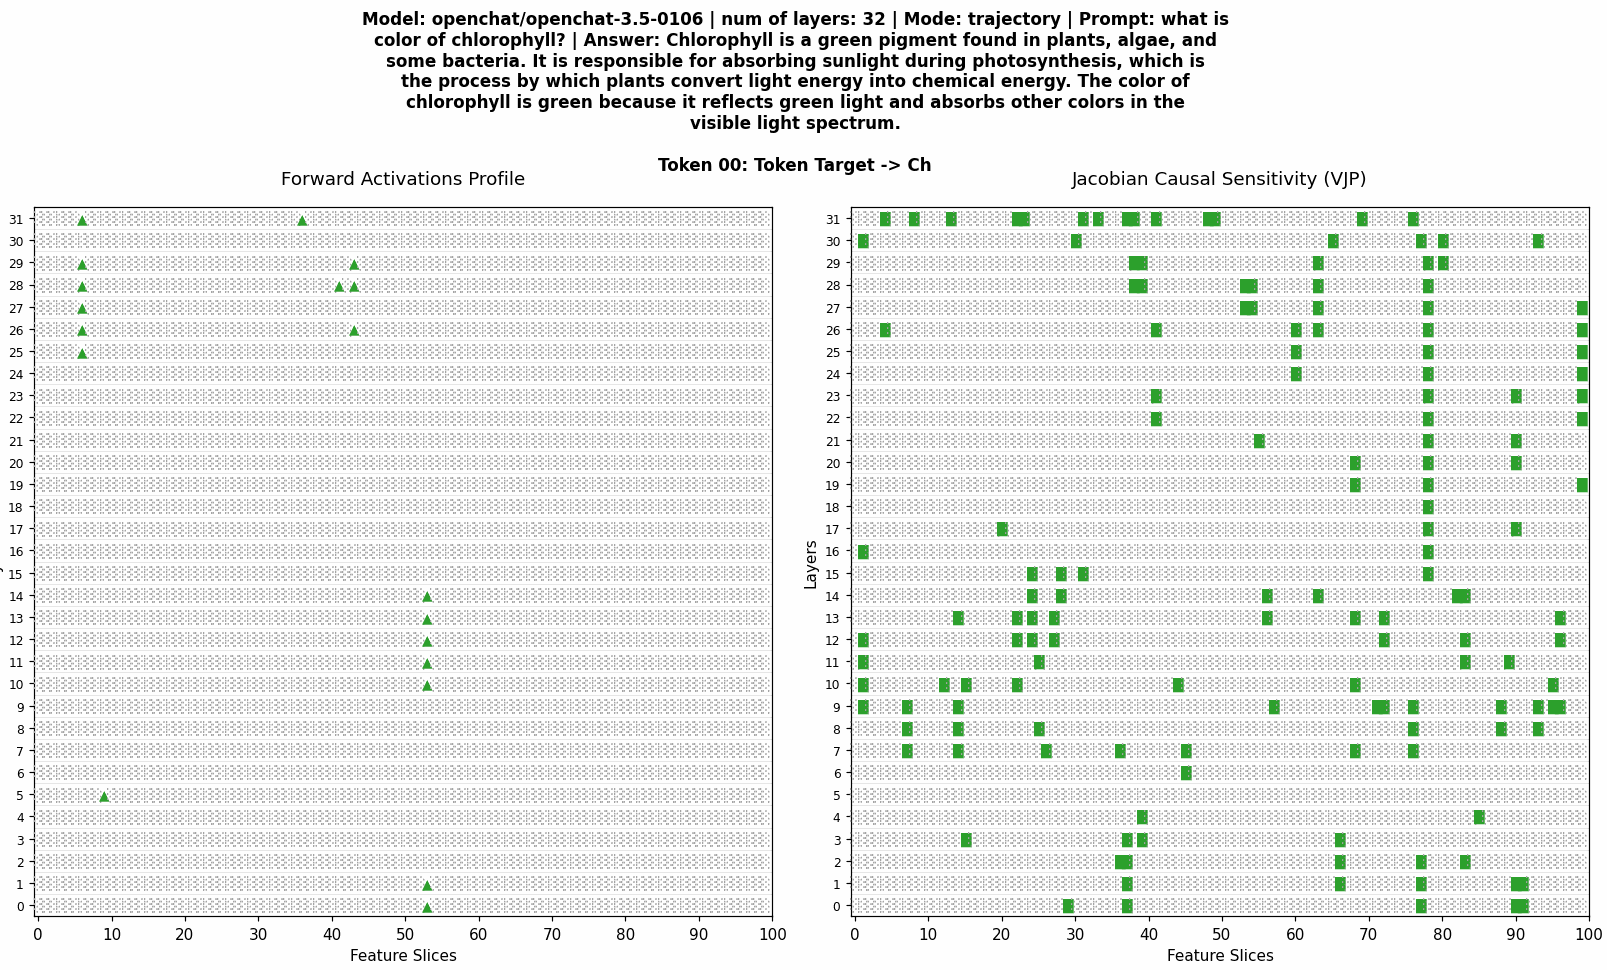
\includegraphics[width=0.95\textwidth]{standard.png}
    \caption{Visual Diagnostics Profile: Token 00 State. ($\mathbf{M}_{\text{std}}$)}
    \label{fig:frame1_large}
\end{figure*}

\begin{figure*}[htbp]
    \centering
    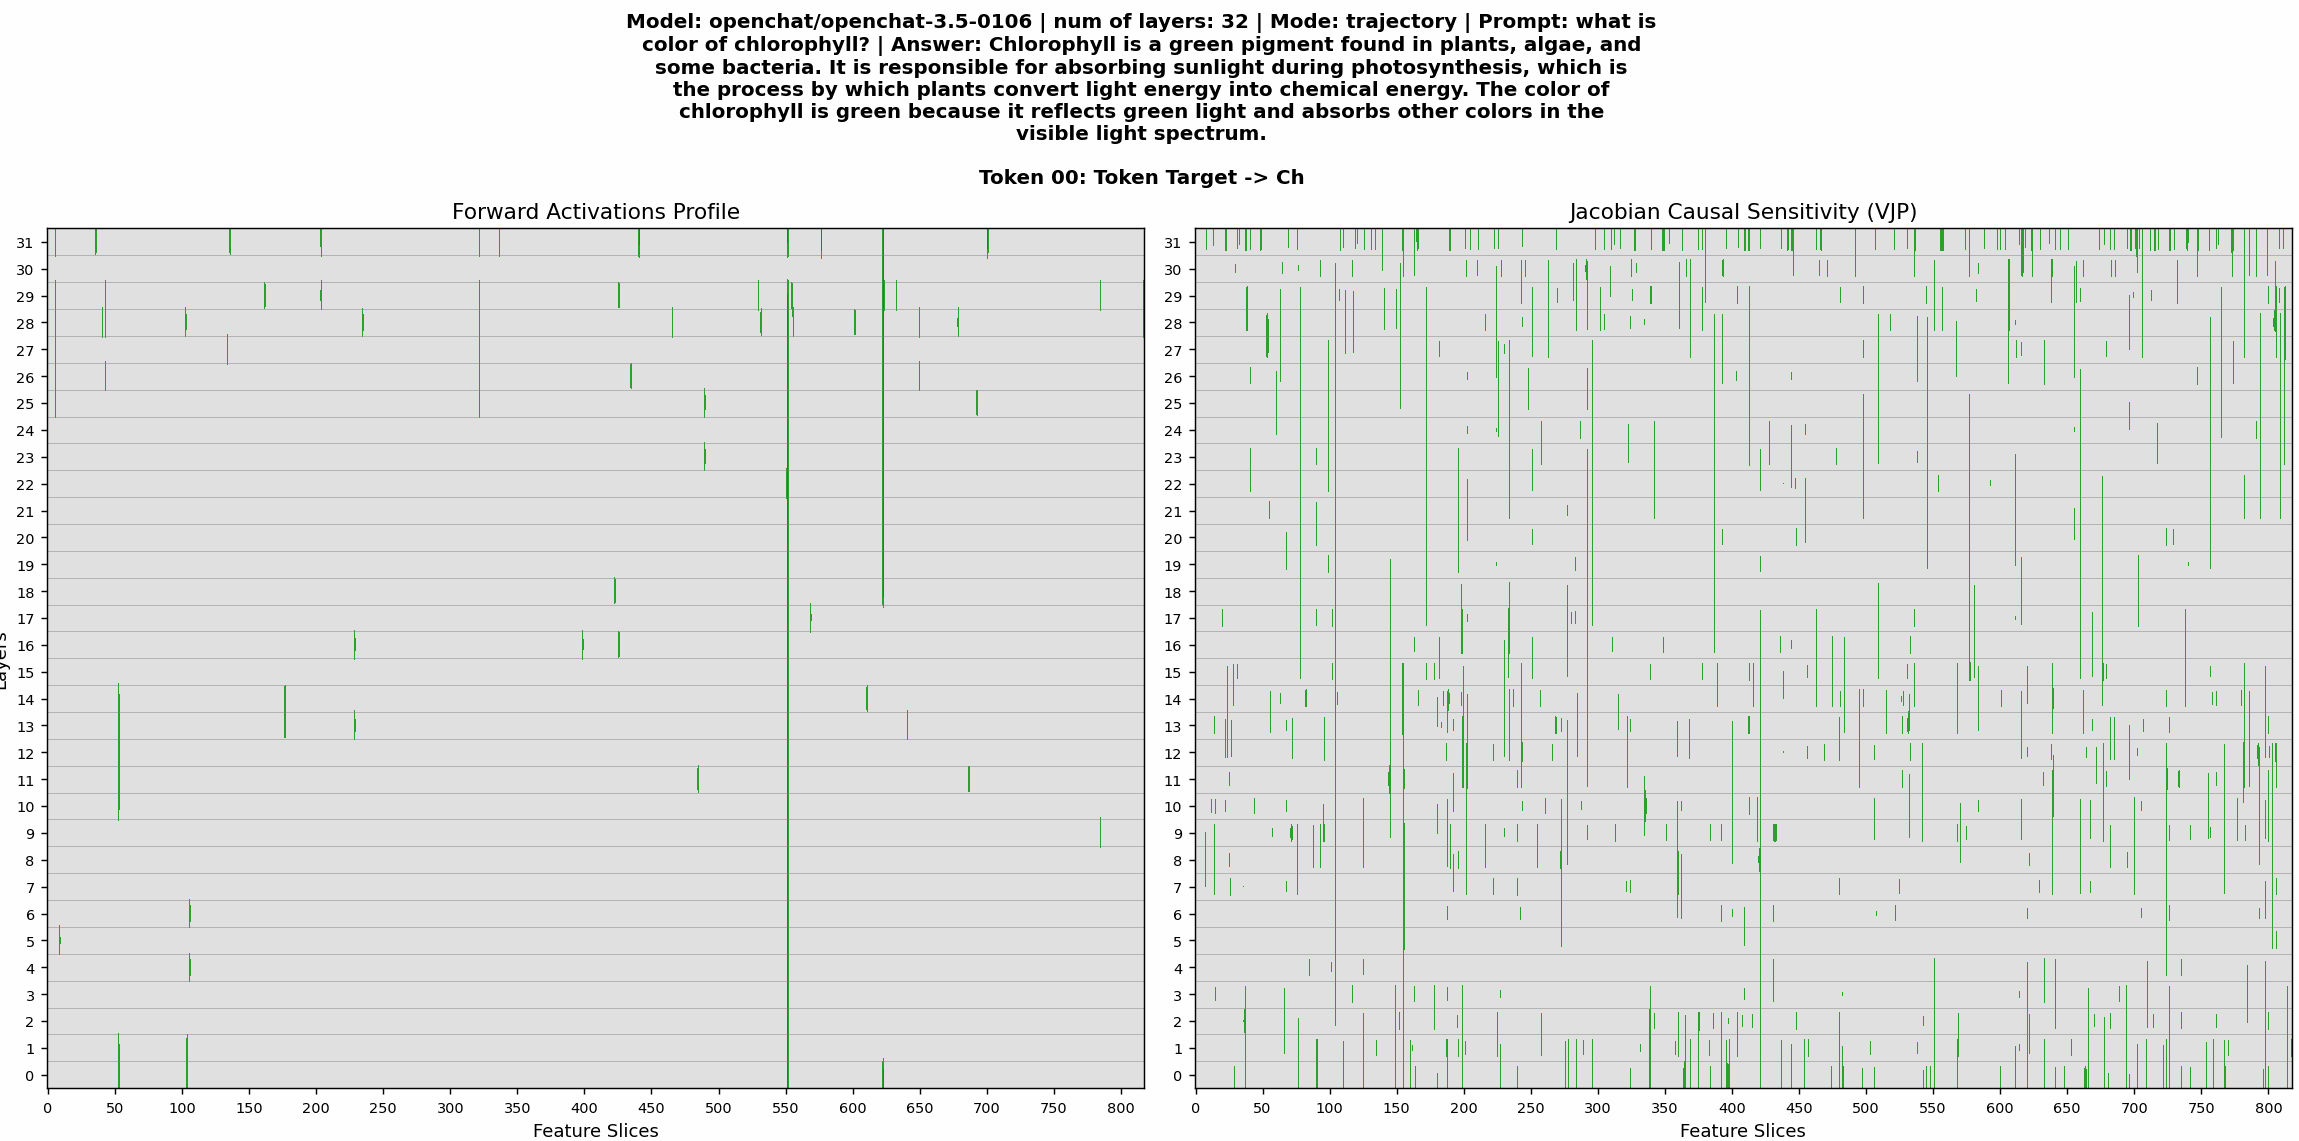
\includegraphics[width=0.95\textwidth]{extended.png}
    \caption{Visual Diagnostics Profile: Token 00 State. ($\mathbf{M}_{\text{exntended}}$)}
    \label{fig:frame2_large}
\end{figure*}

\end{document}
